\begin{frame}{Benchmarks: on Biological Examples}
\begin{columns}
\begin{column}{0.4\textwidth}
\begin{itemize}[<+->]
\item Traditional model checkers: Mole, NuSMV $\to$ \highlight{memory-out}, not listed in the benchmarks
\item Pure static analyzer: Pint~\cite{folschette2015}
\end{itemize}

\vspace{0.3cm}
\begin{itemize}[<+->]
\item Small example: $\lambda$-phage, 4 components
\item Big examples: TCR (T-Cell Receptor, 95 components)
\item EGFR (Epidermal Growth Factor Receptor, 104 components)
\end{itemize}
\end{column}
\begin{column}{0.6\textwidth}
\small
    \centering
    \onslide<3->{\begin{tabular}{|c|c|c|c|}
    \hline
    Model    &  \multicolumn{3}{c|}{$\lambda$-phage}\\
    \hline
    Inputs    & 4 & Outputs& 4\\
    \hline
    Total tests&\multicolumn{3}{c|}{$2^4\times 4=64$}\\
    \hline
    Analyzer  &  Pint  &  \textbf{PermReach}   &\textbf{ASPReach}\\
    \hline
    Reachable & 36(56\%)& \multicolumn{2}{c|}{38(59\%)} \\
    \hline
    Unreachable&\multicolumn{3}{c|}{26(41\%)}\\
    \hline
    \textbf{Inconclusive} &\textcolor{red}{\textbf{2(3\%)}}&\multicolumn{2}{c|}{\textcolor{blue}{\textbf{0(0\%)}}}\\
    \hline
    Total time & \multicolumn{3}{c|}{$<1$s}\\
    \hline
\onslide<4->     Model    &  \multicolumn{3}{c|}{TCR}\\
    \hline
    Inputs    & 3 & Outputs& 5\\
    \hline
    Total tests&\multicolumn{3}{c|}{$2^3\times 5=40$}\\
    \hline
    Analyzer  &  Pint  &  \textbf{PermReach}   &\textbf{ASPReach}\\
    \hline
    Reachable & \multicolumn{3}{c|}{16(40\%)} \\
    \hline
    Unreachable&\multicolumn{3}{c|}{24(60\%)} \\
    \hline
    \textbf{Inconclusive} &\multicolumn{3}{c|}{\textcolor{blue}{\textbf{0(0\%)}}} \\
    \hline
    Total time &  7s     &0.85s  &  40s        \\
    \hline
\onslide<5->     Model    &  \multicolumn{3}{c|}{EGFR}\\
    \hline
    Inputs    & 13 & Outputs& 12\\
    \hline
    Total tests&\multicolumn{3}{c|}{$2^{13}\times 12=98,304$}\\
    \hline
    Analyzer  &  Pint  &  \textbf{PermReach}   &\textbf{ASPReach}\\
    \hline
    Reachable & 64,282(65.4\%)  & \multicolumn{2}{c|}{74,268(75.5\%)} \\
    \hline
    Unreachable&\multicolumn{3}{c|}{24,036(24.5\%)}\\
    \hline
    \textbf{Inconclusive} &\textcolor{red}{\textbf{9,986(10.1\%)}}&\multicolumn{2}{c|}{\textcolor{blue}{\textbf{0(0\%)}}}   \\
    \hline
    Total time & \textbf{9h50min}      & \textbf{15min31s}         & \textbf{3h46min} \\
    \hline
    \end{tabular}
    }
\end{column}
\end{columns}
\end{frame}

\begin{frame}{Benchmarks: on Random Examples}
\onslide<1->{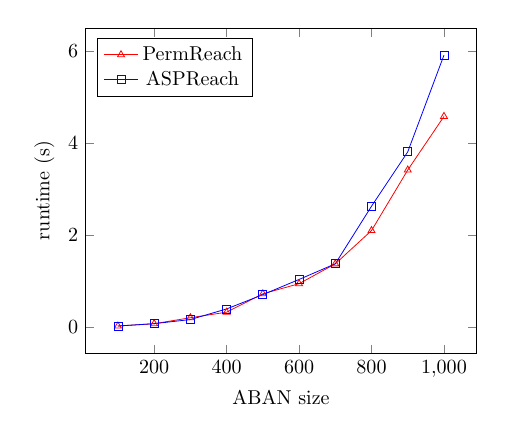
\begin{tikzpicture}[scale=0.725]
    \begin{axis}[xlabel=ABAN size,ylabel=runtime (s),legend pos=north west]
       \addplot[mark=triangle,color=red] coordinates{
        (100,0.029)
        (200,0.079)
        (300,0.209)
        (400,0.330)
        (500,0.729)
        (600,0.948)
        (700,1.379)
        (800,2.102)
        (900,3.416)
        (1000,4.58)
        };
        \addlegendentry{PermReach}
       \addplot[mark=square,color=blue] coordinates{
        (100,0.03)
        (200,0.08)
        (300,0.17)
        (400,0.40)
        (500,0.71)
        (600,1.04)
        (700,1.38)
        (800,2.63)
        (900,3.81)
        (1000,5.91)       
        };
        \addlegendentry{ASPReach}
    \end{axis}
\end{tikzpicture}}
\onslide<2->{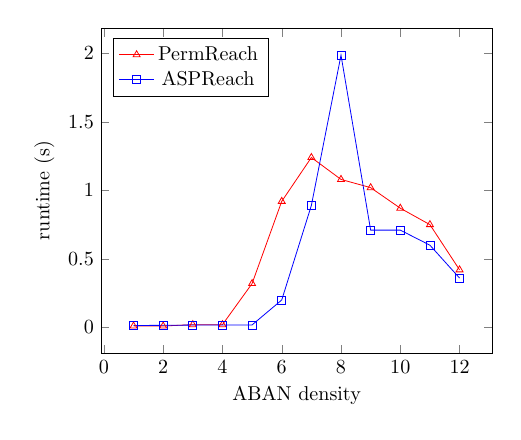
\begin{tikzpicture}[scale=0.725]
\begin{axis}[xlabel=ABAN density,ylabel=runtime (s),legend pos=north west]
\addplot[mark=triangle,color=red] coordinates {
        (1,0.01)
        (2,0.01)
        (3,0.02)
        (4,0.02)
        (5,0.32)
        (6,0.92)
        (7,1.24)
        (8,1.08)
        (9,1.02)
        (10,0.87)
        (11,0.75)
        (12,0.42)
    };
\addlegendentry{PermReach};
       \addplot[mark=square,color=blue] coordinates{
        (1,0.014)
        (2,0.015)
        (3,0.017)
        (4,0.017)
        (5,0.018)
        (6,0.2)
        (7,0.89)
        (8,1.987)
        (9,0.710)
        (10,0.71)
        (11,0.6)
        (12,0.36)    
        };
        \addlegendentry{ASPReach}
\end{axis}
\end{tikzpicture}}

\vspace{0.2cm}
\begin{columns}
\begin{column}{0.5\textwidth}
\centering
\onslide<1->{$$\rm{density}=\dfrac{\#\rm{transitions}}{\#\rm{automata}}$$

Fixing $\rm{density}=3$}
\end{column}
\begin{column}{0.5\textwidth}
\onslide<2->{
\centering
Fixing $\#\rm{automata}=20$
}
\end{column}
\end{columns}
\end{frame}